% Options for packages loaded elsewhere
% Options for packages loaded elsewhere
\PassOptionsToPackage{unicode}{hyperref}
\PassOptionsToPackage{hyphens}{url}
\PassOptionsToPackage{dvipsnames,svgnames,x11names}{xcolor}
%
\documentclass[
  spanish,
  a4paper,
]{scrreport}
\usepackage{xcolor}
\usepackage{amsmath,amssymb}
\setcounter{secnumdepth}{5}
\usepackage{iftex}
\ifPDFTeX
  \usepackage[T1]{fontenc}
  \usepackage[utf8]{inputenc}
  \usepackage{textcomp} % provide euro and other symbols
\else % if luatex or xetex
  \usepackage{unicode-math} % this also loads fontspec
  \defaultfontfeatures{Scale=MatchLowercase}
  \defaultfontfeatures[\rmfamily]{Ligatures=TeX,Scale=1}
\fi
\usepackage{lmodern}
\ifPDFTeX\else
  % xetex/luatex font selection
\fi
% Use upquote if available, for straight quotes in verbatim environments
\IfFileExists{upquote.sty}{\usepackage{upquote}}{}
\IfFileExists{microtype.sty}{% use microtype if available
  \usepackage[]{microtype}
  \UseMicrotypeSet[protrusion]{basicmath} % disable protrusion for tt fonts
}{}
\makeatletter
\@ifundefined{KOMAClassName}{% if non-KOMA class
  \IfFileExists{parskip.sty}{%
    \usepackage{parskip}
  }{% else
    \setlength{\parindent}{0pt}
    \setlength{\parskip}{6pt plus 2pt minus 1pt}}
}{% if KOMA class
  \KOMAoptions{parskip=half}}
\makeatother
% Make \paragraph and \subparagraph free-standing
\makeatletter
\ifx\paragraph\undefined\else
  \let\oldparagraph\paragraph
  \renewcommand{\paragraph}{
    \@ifstar
      \xxxParagraphStar
      \xxxParagraphNoStar
  }
  \newcommand{\xxxParagraphStar}[1]{\oldparagraph*{#1}\mbox{}}
  \newcommand{\xxxParagraphNoStar}[1]{\oldparagraph{#1}\mbox{}}
\fi
\ifx\subparagraph\undefined\else
  \let\oldsubparagraph\subparagraph
  \renewcommand{\subparagraph}{
    \@ifstar
      \xxxSubParagraphStar
      \xxxSubParagraphNoStar
  }
  \newcommand{\xxxSubParagraphStar}[1]{\oldsubparagraph*{#1}\mbox{}}
  \newcommand{\xxxSubParagraphNoStar}[1]{\oldsubparagraph{#1}\mbox{}}
\fi
\makeatother


\usepackage{longtable,booktabs,array}
\newcounter{none} % for unnumbered tables
\usepackage{calc} % for calculating minipage widths
% Correct order of tables after \paragraph or \subparagraph
\usepackage{etoolbox}
\makeatletter
\patchcmd\longtable{\par}{\if@noskipsec\mbox{}\fi\par}{}{}
\makeatother
% Allow footnotes in longtable head/foot
\IfFileExists{footnotehyper.sty}{\usepackage{footnotehyper}}{\usepackage{footnote}}
\makesavenoteenv{longtable}
\usepackage{graphicx}
\makeatletter
\newsavebox\pandoc@box
\newcommand*\pandocbounded[1]{% scales image to fit in text height/width
  \sbox\pandoc@box{#1}%
  \Gscale@div\@tempa{\textheight}{\dimexpr\ht\pandoc@box+\dp\pandoc@box\relax}%
  \Gscale@div\@tempb{\linewidth}{\wd\pandoc@box}%
  \ifdim\@tempb\p@<\@tempa\p@\let\@tempa\@tempb\fi% select the smaller of both
  \ifdim\@tempa\p@<\p@\scalebox{\@tempa}{\usebox\pandoc@box}%
  \else\usebox{\pandoc@box}%
  \fi%
}
% Set default figure placement to htbp
\def\fps@figure{htbp}
\makeatother



\ifLuaTeX
\usepackage[bidi=basic,shorthands=off]{babel}
\else
\usepackage[bidi=default,shorthands=off]{babel}
\fi
\ifLuaTeX
  \usepackage{selnolig} % disable illegal ligatures
\fi


\setlength{\emergencystretch}{3em} % prevent overfull lines

\providecommand{\tightlist}{%
  \setlength{\itemsep}{0pt}\setlength{\parskip}{0pt}}



 


%\newfontfamily\Ubuntu[Mapping=tex-text]{Ubuntu}
\usepackage{pgfplots}
\usetikzlibrary{arrows.meta,arrows}
\usetikzlibrary{angles,quotes}
\pgfplotsset{grid style={dashed,mygray}}
% Colors
\definecolor{myblue}{rgb}{0.067,0.529,0.871}
\definecolor{mypurple}{rgb}{0.859,0.071,0.525}
\definecolor{myred}{rgb}{1.0, 0.13, 0.32}
\definecolor{mygreen}{rgb}{0.01, 0.75, 0.24}
\definecolor{myblack}{gray}{0.1}
\definecolor{mygray}{gray}{0.8}
\makeatletter
\@ifpackageloaded{tcolorbox}{}{\usepackage[skins,breakable]{tcolorbox}}
\@ifpackageloaded{fontawesome5}{}{\usepackage{fontawesome5}}
\definecolor{quarto-callout-color}{HTML}{909090}
\definecolor{quarto-callout-note-color}{HTML}{0758E5}
\definecolor{quarto-callout-important-color}{HTML}{CC1914}
\definecolor{quarto-callout-warning-color}{HTML}{EB9113}
\definecolor{quarto-callout-tip-color}{HTML}{00A047}
\definecolor{quarto-callout-caution-color}{HTML}{FC5300}
\definecolor{quarto-callout-color-frame}{HTML}{acacac}
\definecolor{quarto-callout-note-color-frame}{HTML}{4582ec}
\definecolor{quarto-callout-important-color-frame}{HTML}{d9534f}
\definecolor{quarto-callout-warning-color-frame}{HTML}{f0ad4e}
\definecolor{quarto-callout-tip-color-frame}{HTML}{02b875}
\definecolor{quarto-callout-caution-color-frame}{HTML}{fd7e14}
\makeatother
\makeatletter
\@ifpackageloaded{bookmark}{}{\usepackage{bookmark}}
\makeatother
\makeatletter
\@ifpackageloaded{caption}{}{\usepackage{caption}}
\AtBeginDocument{%
\ifdefined\contentsname
  \renewcommand*\contentsname{Indice de contenidos}
\else
  \newcommand\contentsname{Indice de contenidos}
\fi
\ifdefined\listfigurename
  \renewcommand*\listfigurename{Listado de Figuras}
\else
  \newcommand\listfigurename{Listado de Figuras}
\fi
\ifdefined\listtablename
  \renewcommand*\listtablename{Listado de Tablas}
\else
  \newcommand\listtablename{Listado de Tablas}
\fi
\ifdefined\figurename
  \renewcommand*\figurename{Figura}
\else
  \newcommand\figurename{Figura}
\fi
\ifdefined\tablename
  \renewcommand*\tablename{Tabla}
\else
  \newcommand\tablename{Tabla}
\fi
}
\@ifpackageloaded{float}{}{\usepackage{float}}
\floatstyle{ruled}
\@ifundefined{c@chapter}{\newfloat{codelisting}{h}{lop}}{\newfloat{codelisting}{h}{lop}[chapter]}
\floatname{codelisting}{Listado}
\newcommand*\listoflistings{\listof{codelisting}{Listado de Listados}}
\usepackage{amsthm}
\theoremstyle{definition}
\newtheorem{definition}{Definición}[chapter]
\theoremstyle{definition}
\newtheorem{example}{Ejemplo}[chapter]
\theoremstyle{remark}
\AtBeginDocument{\renewcommand*{\proofname}{Prueba}}
\newtheorem*{remark}{Observación}
\newtheorem*{solution}{Solución}
\newtheorem{refremark}{Observación}[chapter]
\newtheorem{refsolution}{Solución}[chapter]
\makeatother
\makeatletter
\makeatother
\makeatletter
\@ifpackageloaded{caption}{}{\usepackage{caption}}
\@ifpackageloaded{subcaption}{}{\usepackage{subcaption}}
\makeatother
\usepackage{bookmark}
\IfFileExists{xurl.sty}{\usepackage{xurl}}{} % add URL line breaks if available
\urlstyle{same}
\hypersetup{
  pdftitle={Manual de Epidemiología},
  pdfauthor={Alfredo Sánchez Alberca},
  pdflang={es},
  colorlinks=true,
  linkcolor={blue},
  filecolor={Maroon},
  citecolor={Blue},
  urlcolor={Blue},
  pdfcreator={LaTeX via pandoc}}


\title{Manual de Epidemiología}
\usepackage{etoolbox}
\makeatletter
\providecommand{\subtitle}[1]{% add subtitle to \maketitle
  \apptocmd{\@title}{\par {\large #1 \par}}{}{}
}
\makeatother
\subtitle{para Ciencias de la Salud}
\author{Alfredo Sánchez Alberca}
\date{2026-08-31}
\begin{document}
\begin{titlepage}

%\AddToShipoutPicture*{\put(0,0){\includegraphics[scale=0.8]{img/background2}}} % Imagen de fondo, requiere el paquete eso-pic.
\begin{center}
\vspace*{5cm}

\Huge
{\textbf{\textsf{Manual de Epidemiología}}}

\vspace{0.5cm}
\LARGE
{\textbf{\textsf{para Ciencias de la Salud}}}

\vspace{1.5cm}


\includegraphics[width=0.4\textwidth]{img/logos/sticker.png}
\end{center}

\vfill

\begin{flushleft}
\begin{tabular}{ll}

\includegraphics[width=0.1\textwidth]{img/logos/aprendeconalf.png} & \parbox[b]{5cm}{\Large\textsf{Alfredo
Sánchez
Alberca}\\ \textsf{asalber@ceu.es} \\ \textsf{https://aprendeconalf.es}}
\end{tabular}
\end{flushleft}
\end{titlepage}
\renewcommand*\contentsname{Indice de contenidos}
{
\setcounter{tocdepth}{2}
\tableofcontents
}

\bookmarksetup{startatroot}

\chapter*{Prefacio}\label{prefacio}
\addcontentsline{toc}{chapter}{Prefacio}

\markboth{Prefacio}{Prefacio}

¡Bienvenida/os al manual de Epidemiología!

Este libro es una introducción a los conceptos básicos de la
Epidemiología para alumnos de grados en Ciencias de la Salud.

La pandemia de la COVID-19 puso en boca de todos un montón de términos
técnicos de la Epidemiología (prevalencia, incidencia, riesgo relativo,
sensibilidad, falsos positivos, etc.) que, con demasiada frecuencia, se
utilizan de manera errónea, incluso por los propios medios de
comunicación, generando confusión en la población no experta.

El objetivo de este manual es explicar los principales índices
epidemiológicos utilizados en el control de las enfermedades e ilustrar
su uso con ejemplos de aplicación. Como todos ellos se basan en el
cálculo de probabilidades, el libro comienza repasando el concepto de
probabilidad y sus principales propiedades, para después presentar

\begin{itemize}
\tightlist
\item
  las medidas de frecuencia de una enfermedad (prevalencia e
  incidencia),
\item
  las medidas de asociación entre un factor de exposición y una
  enfermedad (riesgo relativo y odds ratio), y
\item
  las medidas de fiabilidad de los tests diagnósticos (sensibilidad,
  especificidad, valores predictivos y curva ROC).
\end{itemize}

Este libro se complementa con los siguientes recursos:

\begin{itemize}
\tightlist
\item
  \href{https://aprendeconalf.es/estadistica-manual/}{Manual de
  Estadística}
\item
  \href{https://aprendeconalf.es/estadistica-ejercicios/}{Colección de
  problemas resueltos}
\item
  \href{https://aprendeconalf.es/estadistica-practicas-r/}{Prácticas de
  Estadística con R}
\item
  \href{http://nube.aprendeconalf.es/shiny/diagnostic-test/}{Aplicación
  para el estudio de test diagnósticos}
\end{itemize}

\section*{Licencia}\label{licencia}
\addcontentsline{toc}{section}{Licencia}

\markright{Licencia}

Esta obra está bajo una licencia Reconocimiento -- No comercial --
Compartir bajo la misma licencia 3.0 España de Creative Commons. Para
ver una copia de esta licencia, visite
\url{https://creativecommons.org/licenses/by-nc-sa/3.0/es/}.

Con esta licencia eres libre de:

\begin{itemize}
\tightlist
\item
  Copiar, distribuir y mostrar este trabajo.
\item
  Realizar modificaciones de este trabajo.
\end{itemize}

Bajo las siguientes condiciones:

\begin{itemize}
\item
  \textbf{Reconocimiento} Debe reconocer los créditos de la obra de la
  manera especificada por el autor o el licenciador (pero no de una
  manera que sugiera que tiene su apoyo o apoyan el uso que hace de su
  obra).
\item
  \textbf{No comercial} No puede utilizar esta obra para fines
  comerciales.
\item
  \textbf{Compartir bajo la misma licencia} Si altera o transforma esta
  obra, o genera una obra derivada, sólo puede distribuir la obra
  generada bajo una licencia idéntica a ésta.
\end{itemize}

Al reutilizar o distribuir la obra, tiene que dejar bien claro los
términos de la licencia de esta obra.

Estas condiciones pueden no aplicarse si se obtiene el permiso del
titular de los derechos de autor.

Nada en esta licencia menoscaba o restringe los derechos morales del
autor.

\bookmarksetup{startatroot}

\chapter{Introducción a la Epidemiología}\label{sec-introduccion}

\section{¿Qué es la Epidemiología?}\label{quuxe9-es-la-epidemiologuxeda}

La palabra \emph{epidemiología} viene del griego \emph{epi} (sobre),
\emph{demos} (gente) y \emph{logos} (estudio), es decir, el estudio de
lo que le ocurre a las poblaciones.

\begin{definition}[Epidemiología]\protect\hypertarget{def-epidemiologia}{}\label{def-epidemiologia}

En el ámbito de la salud pública, la \emph{Epidemiología} es la rama de
la Medicina que se encarga del estudio de la distribución y las causas
de los eventos relacionados con la salud (normalmente enfermedades) en
las poblaciones, y de la aplicación de este estudio al control de los
problemas de salud pública.

\end{definition}

\begin{figure}

\centering{


\includegraphics[width=0.8\linewidth,height=\textheight,keepaspectratio]{img/introduccion/detective.png}

}

\caption{\label{fig-detective}El epidemiólogo trabaja como un detective
que busca las causas de una enfermedad}

\end{figure}%

Obsérvese que, a diferencia de la Medicina clínica, que se ocupa del
diagnóstico y el tratamiento de un paciente concreto, la Epidemiología
estudia siempre \emph{poblaciones}. Sus dos preguntas fundamentales son:

\begin{itemize}
\tightlist
\item
  ¿Cuánta enfermedad hay y cómo se distribuye? (\emph{Epidemiología
  descriptiva})
\item
  ¿Qué factores la causan o la previenen? (\emph{Epidemiología
  analítica})
\end{itemize}

Debido a la epidemia provocada por el coronavirus, la Epidemiología se
ha convertido en una de las ramas de la Medicina que más interés
despiertan.

\begin{figure}

\centering{


\includegraphics[width=0.6\linewidth,height=\textheight,keepaspectratio]{img/introduccion/fernando-simon.jpg}

}

\caption{\label{fig-fernando-simon}Fernando Simón, director del Centro
de Coordinación de Alertas y Emergencias Sanitarias durante la pandemia
de COVID-19}

\end{figure}%

Sin embargo, mucho antes de la COVID, la Epidemiología ya había servido
en otros momentos históricos para resolver o controlar algunos de los
problemas de salud pública más serios que ha enfrentado la humanidad.

\subsection{Algunos descubrimientos
históricos}\label{algunos-descubrimientos-histuxf3ricos}

\begin{itemize}
\tightlist
\item
  \textbf{1854}: John Snow determina que la causa de la epidemia de
  cólera que asolaba Londres era que el agua estaba contaminada con
  heces.
\item
  \textbf{1898}: Ronald Ross averigua que el transmisor de la malaria es
  el mosquito \emph{Anopheles}.
\item
  \textbf{1950}: Se descubre que fumar es el principal factor de riesgo
  del cáncer de pulmón.
\item
  \textbf{1954}: Se valida la primera vacuna contra la poliomielitis (la
  de Jonas Salk).
\item
  \textbf{1970}: Se observa que el ejercicio físico y una dieta sana
  reducen el riesgo de sufrir un infarto.
\item
  \textbf{1983}: Robert Gallo, Luc Montagnier y Françoise Barré-Sinoussi
  identifican el virus que causa el SIDA. Poco después se observó que el
  riesgo de contraer el VIH aumentaba con ciertas prácticas sexuales y
  con el consumo de algunos tipos de drogas.
\item
  \textbf{2020}: Y llegó la COVID\ldots{}
\end{itemize}

\section{El lenguaje de la
Epidemiología}\label{el-lenguaje-de-la-epidemiologuxeda}

En estos tiempos de pandemia un montón de términos técnicos de la
Epidemiología se han convertido en lugares comunes gracias a los medios
de comunicación.

\begin{figure}

\centering{

\pandocbounded{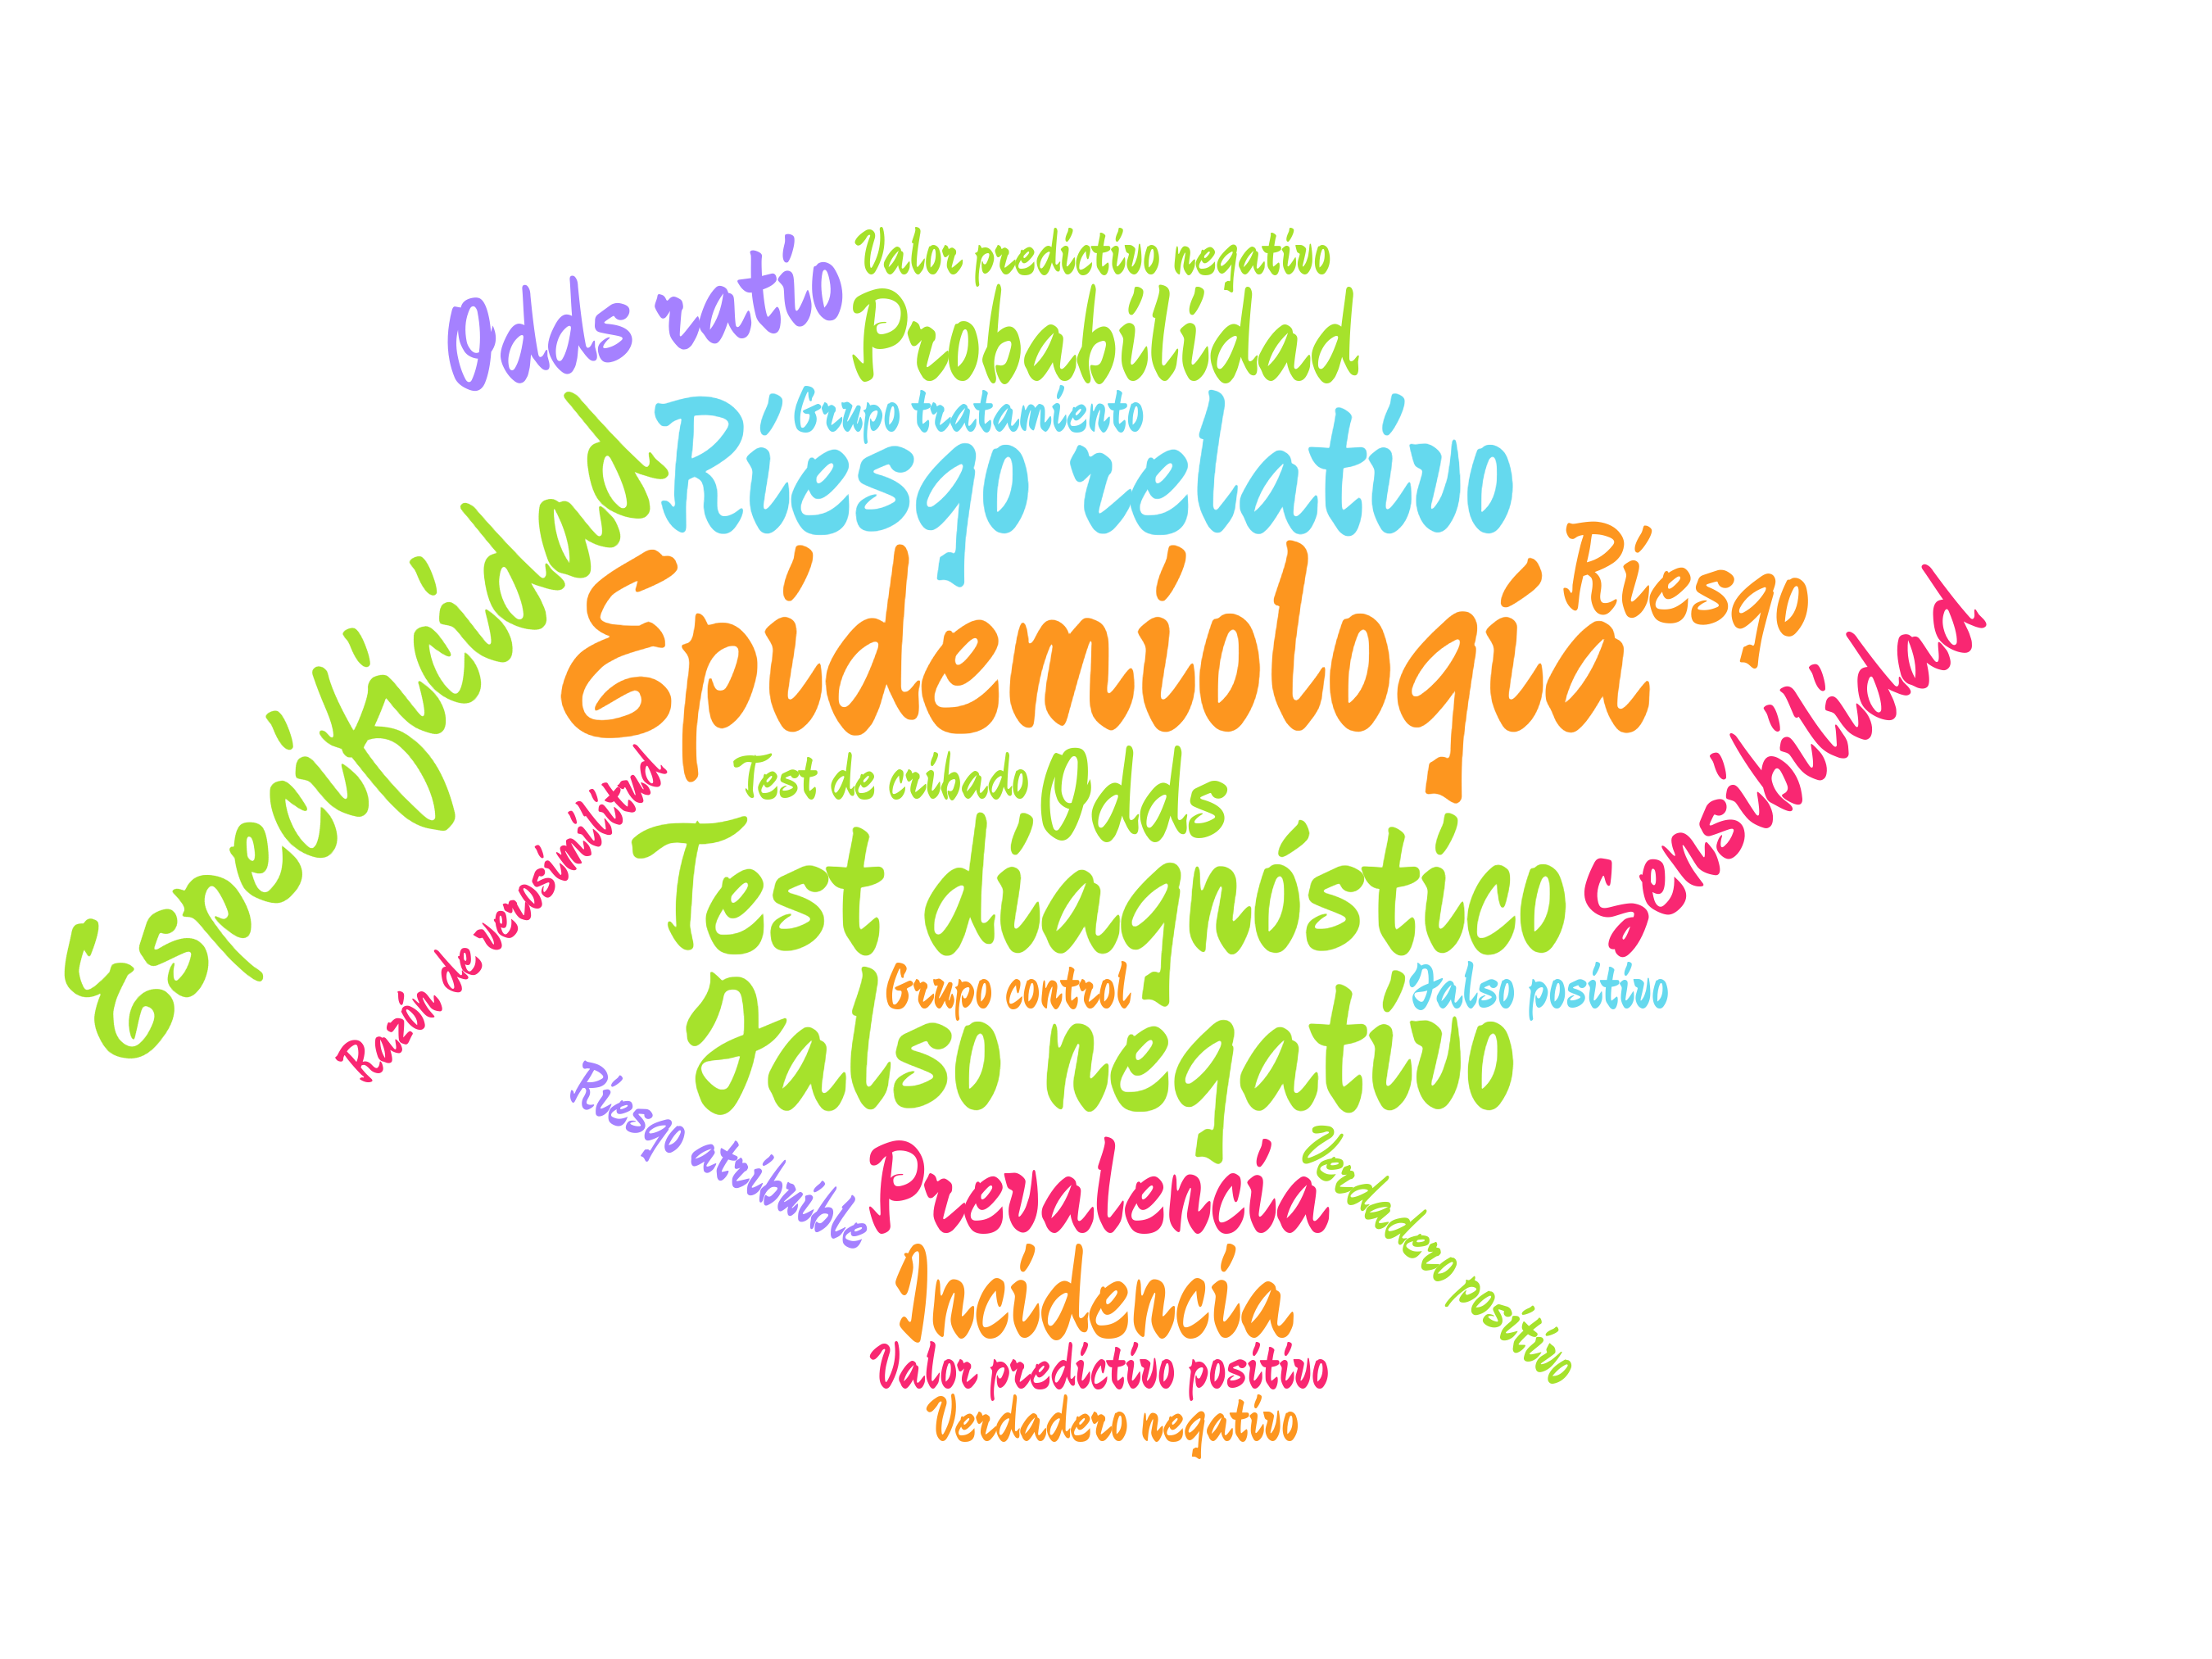
\includegraphics[keepaspectratio]{img/introduccion/wordcloud.png}}

}

\caption{\label{fig-wordcloud}Términos epidemiológicos habituales en los
medios de comunicación}

\end{figure}%

Sin embargo, muchos de estos términos se utilizan de manera errónea,
incluso por los propios medios de comunicación, y generan confusión en
la población no experta. En este manual se explican los principales
conceptos epidemiológicos usados en el control de enfermedades como la
COVID y se ilustra su uso con ejemplos de aplicación.

\section{Índices epidemiológicos}\label{uxedndices-epidemioluxf3gicos}

Los índices epidemiológicos que se estudian en este manual pueden
agruparse en tres bloques:

\begin{description}
\item[\textbf{Medidas de frecuencia de una enfermedad}
(Capítulo~\ref{sec-medidas-frecuencia})]
Miden cuánta enfermedad hay en una población.

\begin{itemize}
\tightlist
\item
  Prevalencia.
\item
  Incidencia o riesgo absoluto.
\end{itemize}
\item[\textbf{Medidas de asociación}
(Capítulo~\ref{sec-medidas-asociacion})]
Miden la relación entre la exposición a un factor y la aparición de la
enfermedad.

\begin{itemize}
\tightlist
\item
  Riesgo y odds.
\item
  Riesgo relativo y odds ratio.
\end{itemize}
\item[\textbf{Medidas de fiabilidad de los tests diagnósticos}
(Capítulo~\ref{sec-tests-diagnosticos} y Capítulo~\ref{sec-curva-roc})]
Miden la capacidad de un test para diagnosticar o descartar la
enfermedad.

\begin{itemize}
\tightlist
\item
  Sensibilidad y especificidad.
\item
  Valores predictivos.
\item
  Curva ROC y área bajo la curva.
\end{itemize}
\end{description}

Todos estos índices están basados en el cálculo de probabilidades, por
lo que en el siguiente capítulo se introduce el concepto de probabilidad
y sus principales propiedades.

\bookmarksetup{startatroot}

\chapter{Probabilidad y odds}\label{sec-probabilidad}

Todos los índices epidemiológicos que se estudian en este manual son, en
el fondo, probabilidades o cocientes de probabilidades. Por eso, antes
de definirlos, conviene repasar el concepto de probabilidad, sus
propiedades y su interpretación, así como una forma alternativa de medir
la incertidumbre: el \emph{odds}.

\section{El concepto de probabilidad}\label{el-concepto-de-probabilidad}

A lo largo de la historia ha habido diferentes intentos de definir
matemáticamente el concepto de probabilidad. Quizá la más conocida, y la
primera que se enseña en las escuelas, es la definición clásica de
Laplace.

\begin{definition}[Probabilidad: definición clásica de
Laplace]\protect\hypertarget{def-probabilidad-laplace}{}\label{def-probabilidad-laplace}

Dado un experimento aleatorio con espacio muestral \(\Omega\) en el que
todos los casos posibles son equiprobables, la \emph{probabilidad} de un
suceso \(E\) es

\[P(E)=\frac{|E|}{|\Omega|}=\frac{\mbox{Casos favorables a $E$}}{\mbox{Casos posibles}}\]

\end{definition}

\begin{example}[]\protect\hypertarget{exm-probabilidad-laplace}{}\label{exm-probabilidad-laplace}

Al tirar un dado equilibrado, la probabilidad de sacar un número par
\(E=\{2, 4, 6\}\) es

\[P(E) = \frac{3}{6} = 0.5.\]

\end{example}

Sin embargo, esta definición tiene serios inconvenientes ya que, para
poder usarla, todos los casos posibles del experimento deben tener la
misma probabilidad de ocurrir (\emph{equiprobabilidad}), y esto no suele
ocurrir en la vida real (por ejemplo, no todos los grupos sanguíneos
tienen la misma probabilidad de ocurrir).

Por este motivo, en el ámbito de las Ciencias de la Salud es mucho más
común utilizar la definición de probabilidad basada en el cálculo de
frecuencias.

\begin{definition}[Probabilidad: definición
frecuentista]\protect\hypertarget{def-probabilidad-frecuentista}{}\label{def-probabilidad-frecuentista}

La \emph{probabilidad} de un suceso \(E\) se aproxima mediante su
frecuencia relativa en una muestra de tamaño \(n\),

\[P(E)\approx f_E = \frac{n_E}{n}=\frac{\mbox{Frecuencia absoluta del suceso}}{\mbox{Tamaño muestral}}\]

\end{definition}

\begin{example}[]\protect\hypertarget{exm-probabilidad-frecuentista}{}\label{exm-probabilidad-frecuentista}

Se ha aplicado un tratamiento a 100 personas y se han curado 75.
Entonces, la probabilidad de curación del tratamiento es

\[P(E) = \frac{75}{100} = 0.75 \Rightarrow 75\%.\]

\end{example}

\begin{tcolorbox}[enhanced jigsaw, arc=.35mm, bottomrule=.15mm, bottomtitle=1mm, breakable, colback=white, colbacktitle=quarto-callout-warning-color!10!white, colframe=quarto-callout-warning-color-frame, coltitle=black, left=2mm, leftrule=.75mm, opacityback=0, opacitybacktitle=0.6, rightrule=.15mm, title=\textcolor{quarto-callout-warning-color}{\faExclamationTriangle}\hspace{0.5em}{Advertencia}, titlerule=0mm, toprule=.15mm, toptitle=1mm]

La definición frecuentista no permite calcular el valor exacto de la
probabilidad de un suceso, sino tan solo una aproximación, que será
mejor cuanto mayor sea el tamaño de la muestra.

\end{tcolorbox}

\subsection{Algunas propiedades de la
probabilidad}\label{algunas-propiedades-de-la-probabilidad}

\begin{itemize}
\tightlist
\item
  Una probabilidad es un número real entre 0 y 1:
\end{itemize}

\[0\leq P(E)\leq 1.\]

\begin{itemize}
\tightlist
\item
  La suma de las probabilidades de todos los casos posibles es 1:
\end{itemize}

\[P(\Omega) = P(e_1) + P(e_2) + \cdots + P(e_n) = 1.\]

\begin{itemize}
\tightlist
\item
  La probabilidad de que ocurra lo contrario de un suceso es 1 menos la
  probabilidad del suceso:
\end{itemize}

\[P(\overline E) = 1 - P(E).\]

De este modo, cuanto más probable es que ocurra un suceso, menos
probable es que ocurra su contrario, y viceversa.

\subsection{Interpretación de una
probabilidad}\label{interpretaciuxf3n-de-una-probabilidad}

La probabilidad mide la verosimilitud de un suceso. De manera informal,
se puede decir que la probabilidad mide la creencia o la confianza que
tenemos en la ocurrencia de un suceso.

\begin{tcolorbox}[enhanced jigsaw, arc=.35mm, bottomrule=.15mm, bottomtitle=1mm, breakable, colback=white, colbacktitle=quarto-callout-note-color!10!white, colframe=quarto-callout-note-color-frame, coltitle=black, left=2mm, leftrule=.75mm, opacityback=0, opacitybacktitle=0.6, rightrule=.15mm, title=\textcolor{quarto-callout-note-color}{\faInfo}\hspace{0.5em}{Interpretación}, titlerule=0mm, toprule=.15mm, toptitle=1mm]

\begin{itemize}
\tightlist
\item
  \(P(E) = 0 \Rightarrow\) Mínima verosimilitud (el suceso no ocurre
  nunca).
\item
  \(P(E) = 0.5 \Rightarrow\) Verosimilitud media (máxima incertidumbre).
\item
  \(P(E) = 1 \Rightarrow\) Máxima verosimilitud (el suceso ocurre
  siempre).
\end{itemize}

\end{tcolorbox}

\begin{figure}

\centering{

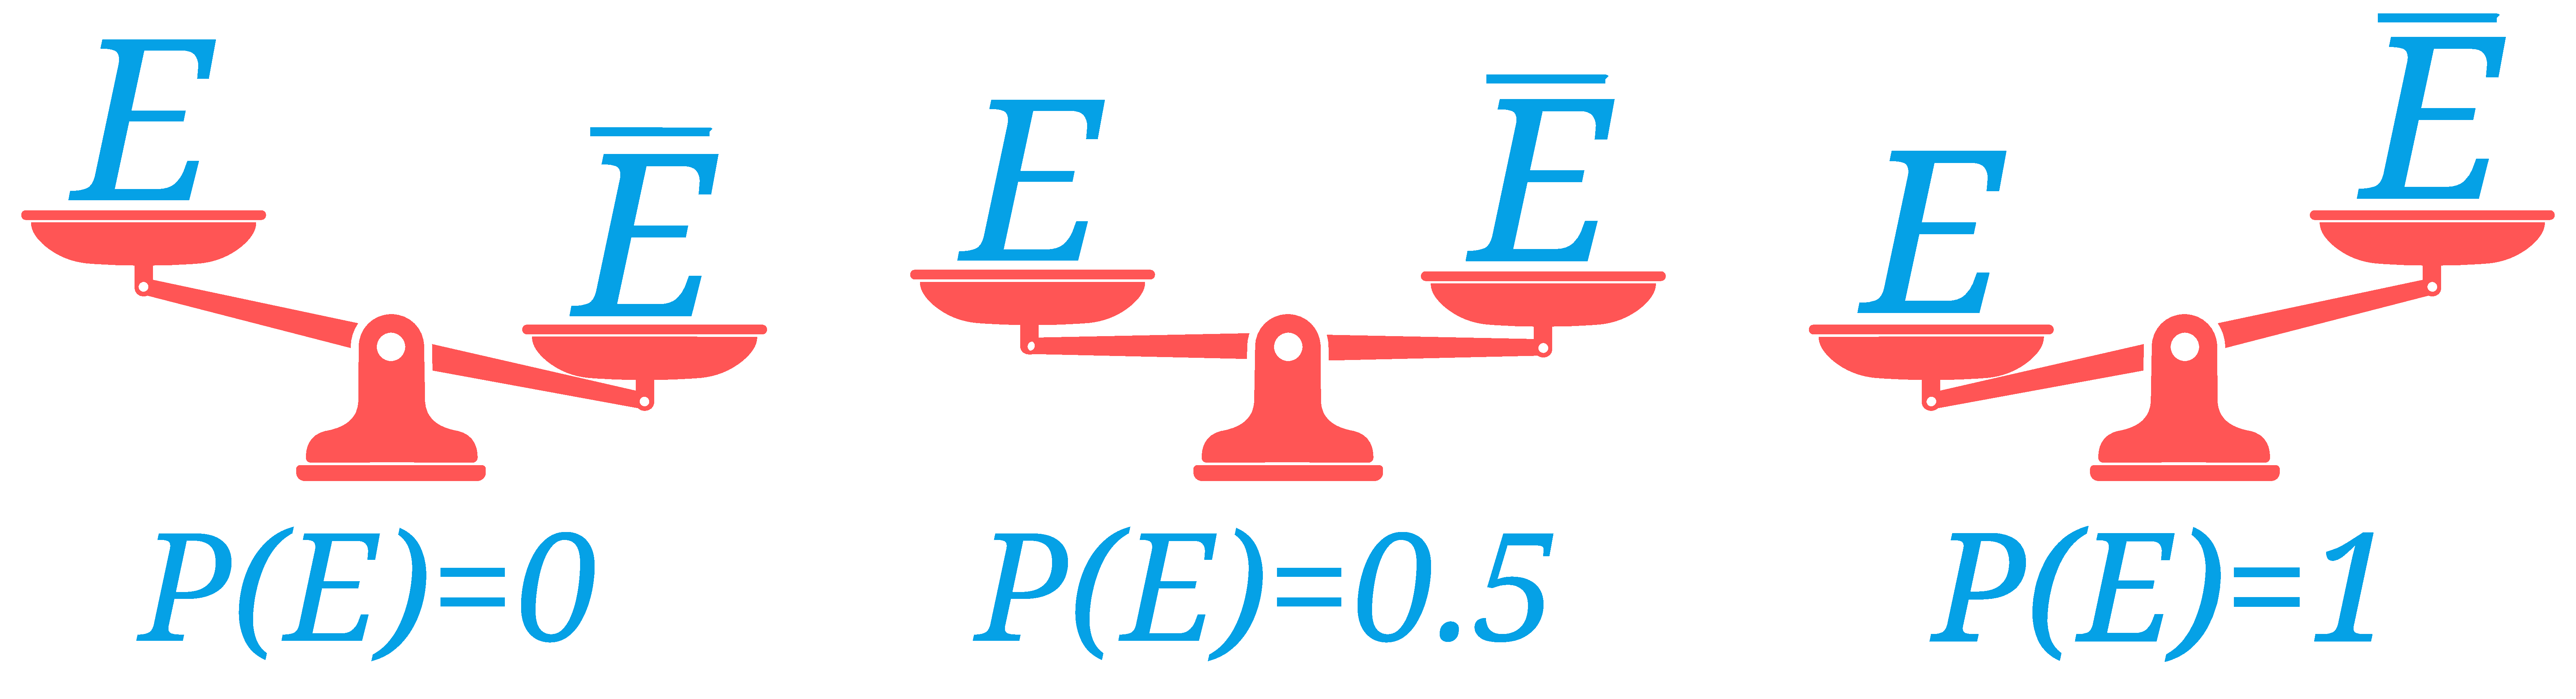
\includegraphics[width=0.9\linewidth,height=\textheight,keepaspectratio]{img/probabilidad/balanza-probabilidad.pdf}

}

\caption{\label{fig-balanza-probabilidad}Escala de interpretación de una
probabilidad}

\end{figure}%

Aunque el concepto de probabilidad es el más extendido en las
aplicaciones que requieren cuantificar la incertidumbre sobre la
ocurrencia de un suceso, existen otras formas de cuantificar esa
incertidumbre, como por ejemplo el \emph{odds}.

\section{El concepto de odds}\label{el-concepto-de-odds}

\begin{definition}[Odds]\protect\hypertarget{def-odds}{}\label{def-odds}

El \emph{odds} de un suceso \(E\) es el cociente entre el número de
casos en los que ocurre \(E\) y el número de casos en los que no ocurre,

\[O(E)=\frac{\mbox{N.º casos con $E$}}{\mbox{N.º casos sin $E$}}=\frac{P(E)}{P(\overline E)}\]

\end{definition}

\begin{example}[]\protect\hypertarget{exm-odds}{}\label{exm-odds}

Se ha aplicado un tratamiento a 100 personas y se han curado 75.
Entonces, el odds de curación del tratamiento es

\[O(E) = \frac{75}{25} = 3,\]

es decir, por cada persona que no se cura hay 3 que se curan.

\end{example}

\begin{tcolorbox}[enhanced jigsaw, arc=.35mm, bottomrule=.15mm, bottomtitle=1mm, breakable, colback=white, colbacktitle=quarto-callout-warning-color!10!white, colframe=quarto-callout-warning-color-frame, coltitle=black, left=2mm, leftrule=.75mm, opacityback=0, opacitybacktitle=0.6, rightrule=.15mm, title=\textcolor{quarto-callout-warning-color}{\faExclamationTriangle}\hspace{0.5em}{Advertencia}, titlerule=0mm, toprule=.15mm, toptitle=1mm]

A diferencia de una probabilidad, un odds puede ser mayor que 1. De
hecho, no tiene cota superior.

\end{tcolorbox}

\subsection{Interpretación de un
odds}\label{interpretaciuxf3n-de-un-odds}

Los odds también permiten cuantificar la verosimilitud de un
suceso\ldots, pero en una escala diferente, ya que se trata de una razón
de probabilidades.

\begin{tcolorbox}[enhanced jigsaw, arc=.35mm, bottomrule=.15mm, bottomtitle=1mm, breakable, colback=white, colbacktitle=quarto-callout-note-color!10!white, colframe=quarto-callout-note-color-frame, coltitle=black, left=2mm, leftrule=.75mm, opacityback=0, opacitybacktitle=0.6, rightrule=.15mm, title=\textcolor{quarto-callout-note-color}{\faInfo}\hspace{0.5em}{Interpretación}, titlerule=0mm, toprule=.15mm, toptitle=1mm]

\begin{itemize}
\tightlist
\item
  \(O(E) = 0 \Rightarrow\) Mínima verosimilitud.
\item
  \(O(E) = 1 \Rightarrow\) Verosimilitud media (máxima incertidumbre).
\item
  \(O(E) = \infty \Rightarrow\) Máxima verosimilitud.
\end{itemize}

\end{tcolorbox}

\begin{figure}

\centering{

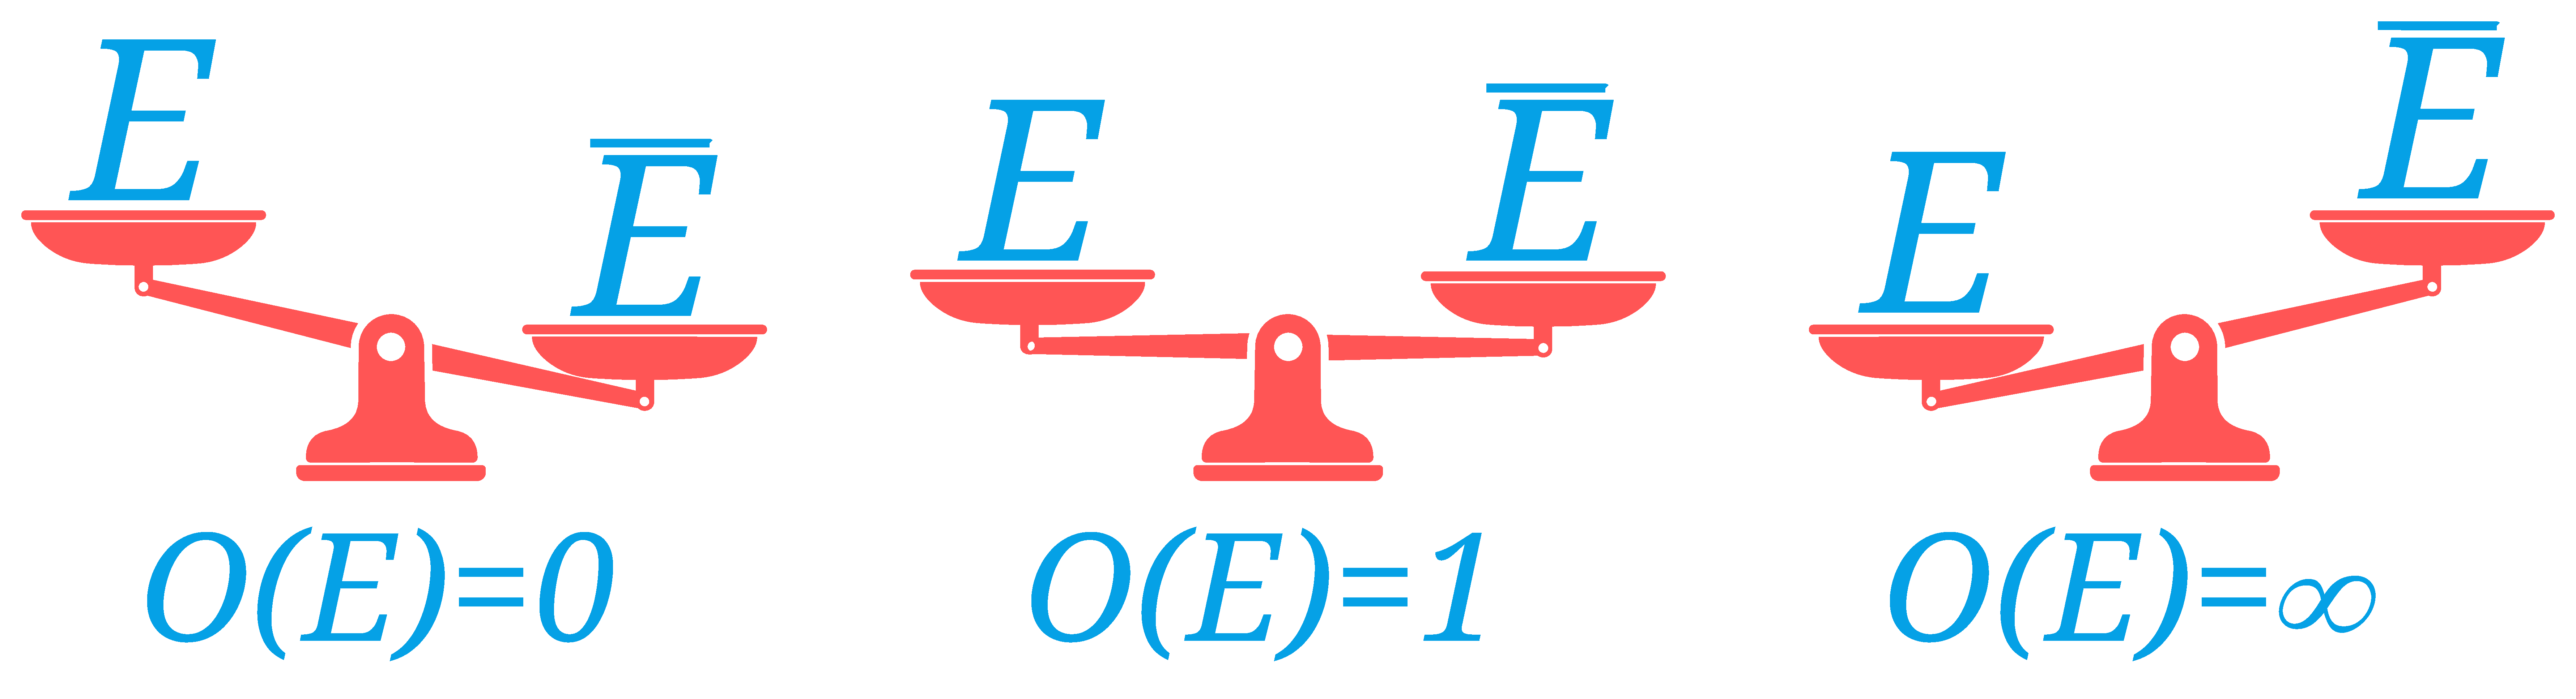
\includegraphics[width=0.9\linewidth,height=\textheight,keepaspectratio]{img/probabilidad/balanza-odds.pdf}

}

\caption{\label{fig-balanza-odds}Escala de interpretación de un odds}

\end{figure}%

\subsection{Conversión de odds en
probabilidades}\label{conversiuxf3n-de-odds-en-probabilidades}

Como el odds es una función de la probabilidad, es posible convertir un
odds en una probabilidad aplicando la siguiente fórmula:

\[\frac{O(E)}{1 + O(E)} = \frac{\dfrac{P(E)}{P(\overline E)}}{1 + \dfrac{P(E)}{P(\overline E)}} = \frac{\dfrac{P(E)}{P(\overline E)}}{\dfrac{P(\overline E) + P(E)}{P(\overline E)}} = P(E).\]

\begin{example}[]\protect\hypertarget{exm-conversion-odds-probabilidad}{}\label{exm-conversion-odds-probabilidad}

Se ha aplicado un tratamiento a 100 personas y se han curado 75, de
manera que

\[O(E) = \frac{75}{25} = 3 \Rightarrow P(E) = \frac{3}{1+3}=0.75.\]

\end{example}

Y, del mismo modo, se puede pasar de una probabilidad a un odds mediante
la fórmula

\[O(E) = \frac{P(E)}{1-P(E)}.\]

\bookmarksetup{startatroot}

\chapter{Medidas de frecuencia de una
enfermedad}\label{sec-medidas-frecuencia}

La primera tarea de la Epidemiología es cuantificar cuánta enfermedad
hay en una población. Para ello se utilizan dos medidas de frecuencia
que se confunden a menudo, pero que responden a preguntas distintas: la
\emph{prevalencia} y la \emph{incidencia}.

\section{Prevalencia}\label{prevalencia}

\begin{definition}[Prevalencia]\protect\hypertarget{def-prevalencia}{}\label{def-prevalencia}

La \emph{prevalencia} de una enfermedad \(E\) es la proporción de
personas que tienen la enfermedad en un momento concreto,

\[\mbox{Prevalencia}(E) = \frac{\mbox{N.º individuos afectados por $E$}}{\mbox{Tamaño poblacional}}\]

\end{definition}

\begin{example}[]\protect\hypertarget{exm-prevalencia}{}\label{exm-prevalencia}

En una muestra de 1000 personas, 150 tenían gripe. La prevalencia de la
gripe es aproximadamente

\[\frac{150}{1000}=0.15 \Rightarrow 15\%.\]

\end{example}

Obsérvese que en el numerador de la prevalencia se cuentan \emph{todos}
los casos existentes en ese instante, tanto los nuevos como los
antiguos.

\section{Incidencia o riesgo
absoluto}\label{incidencia-o-riesgo-absoluto}

\begin{definition}[Incidencia]\protect\hypertarget{def-incidencia}{}\label{def-incidencia}

La \emph{incidencia} o \emph{riesgo absoluto} de una enfermedad \(E\) es
la proporción de nuevos casos durante un periodo determinado (por día,
por semana, por mes, etc.),

\[R(E)=\frac{\mbox{N.º nuevos casos con $E$ en el periodo}}{\mbox{Tamaño de la población en riesgo al comienzo del periodo}}\]

\end{definition}

\begin{example}[]\protect\hypertarget{exm-incidencia}{}\label{exm-incidencia}

Al comienzo del año se tomó una muestra de 1000 personas sin gripe y al
finalizar el año 80 habían tenido gripe. La incidencia de la gripe ese
año fue

\[R(E) = \frac{80}{1000} = 0.08 \Rightarrow 8\%.\]

\end{example}

\begin{tcolorbox}[enhanced jigsaw, arc=.35mm, bottomrule=.15mm, bottomtitle=1mm, breakable, colback=white, colbacktitle=quarto-callout-important-color!10!white, colframe=quarto-callout-important-color-frame, coltitle=black, left=2mm, leftrule=.75mm, opacityback=0, opacitybacktitle=0.6, rightrule=.15mm, title=\textcolor{quarto-callout-important-color}{\faExclamation}\hspace{0.5em}{Importante}, titlerule=0mm, toprule=.15mm, toptitle=1mm]

En la incidencia, el denominador no es el tamaño de la población, sino
el tamaño de la \emph{población en riesgo}, es decir, las personas que
al comienzo del periodo podían enfermar (no se cuentan ni los ya
enfermos ni los inmunizados).

\end{tcolorbox}

\section{Prevalencia frente a
incidencia}\label{prevalencia-frente-a-incidencia}

\begin{longtable}[]{@{}lccc@{}}
\caption{Diferencias entre la prevalencia y la
incidencia}\label{tbl-prevalencia-incidencia}\tabularnewline
\toprule\noalign{}
& Tiempo & Casos & Tipo de estudio \\
\midrule\noalign{}
\endfirsthead
\toprule\noalign{}
& Tiempo & Casos & Tipo de estudio \\
\midrule\noalign{}
\endhead
\bottomrule\noalign{}
\endlastfoot
Prevalencia & Puntual & Nuevos y existentes & Transversal \\
Incidencia & Periodo & Solo nuevos & Longitudinal \\
\end{longtable}

\begin{itemize}
\tightlist
\item
  La prevalencia muestra el número de personas afectadas (la
  \emph{carga} de la enfermedad) y es útil para planificar los recursos
  sanitarios necesarios.
\item
  La incidencia muestra la evolución de la enfermedad y es más útil para
  detectar brotes y estudiar sus causas.
\item
  La incidencia depende sobre todo de la contagiosidad de la enfermedad,
  mientras que la prevalencia depende también de la duración de la
  enfermedad y de lo agresiva que sea.
\end{itemize}

\begin{example}[]\protect\hypertarget{exm-prevalencia-incidencia}{}\label{exm-prevalencia-incidencia}

Una enfermedad crónica como la diabetes o la artrosis tiene una
incidencia prácticamente constante, al depender fundamentalmente de la
edad y no ser contagiosa, y una prevalencia alta, ya que no existe cura
para ella y las personas tampoco mueren a causa de ella, sino que viven
con ella el resto de su vida.

Por otro lado, una enfermedad como el ébola tiene una incidencia
pequeña, al no ser muy contagiosa, y también una prevalencia pequeña, al
ser una enfermedad mortal, ya que casi todas las personas que se
contagian acaban muriendo.

Finalmente, una enfermedad como la COVID tiene una incidencia muy alta,
al ser muy contagiosa, y una prevalencia parecida a la incidencia, ya
que la enfermedad suele acabar en un periodo de dos semanas desde el
contagio (salvo en los casos que necesitan hospitalización).

\end{example}

\section{Algunas consideraciones en el caso de la
COVID}\label{algunas-consideraciones-en-el-caso-de-la-covid}

La incidencia de la COVID se suele dar sobre un periodo de dos semanas
(14 días), aunque no siempre, y por cada 100 000 habitantes.

Los datos son poco precisos y subestiman el riesgo de la COVID:

\begin{itemize}
\tightlist
\item
  Muchos asintomáticos no son detectados.
\item
  La detección de casos se realiza mediante tests diagnósticos que
  tienen un margen de error (falsos positivos y falsos negativos), como
  se verá en el Capítulo~\ref{sec-tests-diagnosticos}.
\item
  Se calcula dividiendo por el tamaño de la población (nuevos casos por
  cada 100 000 habitantes), pero habría que dividir por el tamaño de la
  población en riesgo (sin contar los ya infectados o inmunizados).
\end{itemize}

Los datos oficiales pueden consultarse en la página del
\href{https://www.sanidad.gob.es/profesionales/saludPublica/ccayes/alertasActual/nCov/situacionActual.htm}{Ministerio
de Sanidad}.

Tanto la prevalencia como la incidencia permiten estudiar la magnitud y
la evolución de una enfermedad, pero no permiten analizar sus posibles
causas. Para ello es necesario comparar los riesgos de distintos grupos
de población, que es lo que se verá en el siguiente capítulo.

\bookmarksetup{startatroot}

\chapter{Medidas de asociación}\label{sec-medidas-asociacion}

Tanto la prevalencia como la incidencia permiten estudiar la magnitud y
la evolución de una enfermedad, pero no permiten analizar sus posibles
causas. Cuando se quiere investigar si la exposición a un determinado
factor influye en el desarrollo de una enfermedad hay que comparar los
riesgos de dos grupos:

\begin{itemize}
\tightlist
\item
  \textbf{Grupo tratamiento} \(T\): individuos expuestos al factor.
\item
  \textbf{Grupo control} \(C\): individuos no expuestos al factor.
\end{itemize}

Los resultados del estudio se resumen en una tabla de contingencia como
la siguiente, donde \(E\) es el suceso de padecer la enfermedad y
\(\overline E\) el de no padecerla.

\begin{longtable}[]{@{}lcc@{}}
\caption{Tabla de contingencia de un estudio
epidemiológico}\label{tbl-contingencia}\tabularnewline
\toprule\noalign{}
& \(E\) & \(\overline{E}\) \\
\midrule\noalign{}
\endfirsthead
\toprule\noalign{}
& \(E\) & \(\overline{E}\) \\
\midrule\noalign{}
\endhead
\bottomrule\noalign{}
\endlastfoot
Grupo tratamiento \(T\) & \(a\) & \(b\) \\
Grupo control \(C\) & \(c\) & \(d\) \\
\end{longtable}

A partir de esta tabla se pueden definir dos medidas de asociación entre
el factor y la enfermedad: el \emph{riesgo relativo} y el \emph{odds
ratio}.

\section{Riesgo relativo}\label{riesgo-relativo}

\begin{definition}[Riesgo
relativo]\protect\hypertarget{def-riesgo-relativo}{}\label{def-riesgo-relativo}

El \emph{riesgo relativo} de un suceso \(E\) es el cociente entre el
riesgo del grupo tratamiento y el riesgo del grupo control,

\[RR(E)=\frac{\mbox{Riesgo grupo tratamiento}}{\mbox{Riesgo grupo control}}=\frac{R_T(E)}{R_C(E)}=\frac{a/(a+b)}{c/(c+d)}\]

\end{definition}

\begin{example}[]\protect\hypertarget{exm-riesgo-relativo}{}\label{exm-riesgo-relativo}

Para estudiar la eficacia de una vacuna contra la gripe se ha tomado una
muestra de 500 personas vacunadas y otra de 500 no vacunadas,
obteniéndose los siguientes resultados.

{\def\LTcaptype{none} % do not increment counter
\begin{longtable}[]{@{}lcc@{}}
\toprule\noalign{}
& Gripe \(G\) & No gripe \(\overline{G}\) \\
\midrule\noalign{}
\endhead
\bottomrule\noalign{}
\endlastfoot
Vacunados \(T\) & 20 & 480 \\
No vacunados \(C\) & 80 & 420 \\
\end{longtable}
}

El riesgo relativo de padecer gripe es

\[RR(G) = \frac{20/(20+480)}{80/(80+420)} = 0.25,\]

es decir, el riesgo de padecer gripe en los vacunados es la cuarta parte
del riesgo en los no vacunados.

\end{example}

\subsection{Interpretación del riesgo
relativo}\label{interpretaciuxf3n-del-riesgo-relativo}

\begin{tcolorbox}[enhanced jigsaw, arc=.35mm, bottomrule=.15mm, bottomtitle=1mm, breakable, colback=white, colbacktitle=quarto-callout-note-color!10!white, colframe=quarto-callout-note-color-frame, coltitle=black, left=2mm, leftrule=.75mm, opacityback=0, opacitybacktitle=0.6, rightrule=.15mm, title=\textcolor{quarto-callout-note-color}{\faInfo}\hspace{0.5em}{Interpretación}, titlerule=0mm, toprule=.15mm, toptitle=1mm]

\begin{itemize}
\tightlist
\item
  \(RR=1 \Rightarrow\) No hay asociación entre el suceso y la exposición
  al factor.
\item
  \(RR<1 \Rightarrow\) La exposición al factor disminuye el riesgo del
  suceso (factor de protección).
\item
  \(RR>1 \Rightarrow\) La exposición al factor aumenta el riesgo del
  suceso (factor de riesgo).
\end{itemize}

\end{tcolorbox}

\begin{figure}

\centering{

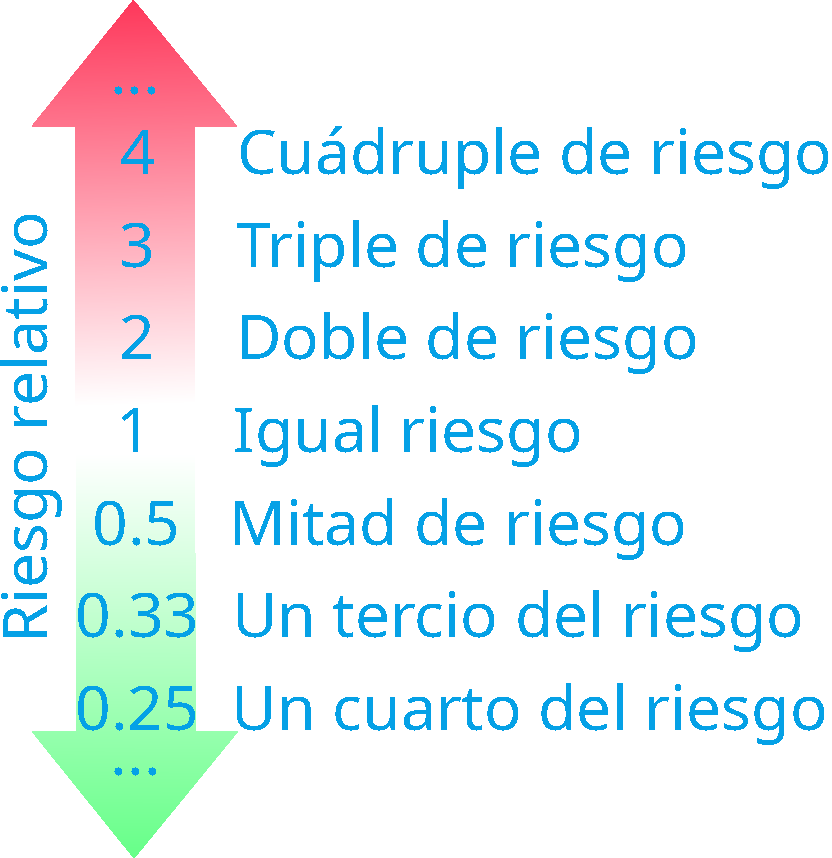
\includegraphics[width=0.65\linewidth,height=\textheight,keepaspectratio]{img/riesgos/escala-riesgo-relativo.pdf}

}

\caption{\label{fig-escala-riesgo-relativo}Escala de interpretación del
riesgo relativo}

\end{figure}%

\section{Odds ratio}\label{odds-ratio}

Del mismo modo que se pueden comparar los riesgos de los grupos
tratamiento y control, se pueden comparar también sus odds.

\begin{definition}[Odds
ratio]\protect\hypertarget{def-odds-ratio}{}\label{def-odds-ratio}

El \emph{odds ratio} o \emph{razón de odds} de un suceso \(E\) es el
cociente entre el odds del grupo tratamiento y el odds del grupo
control,

\[OR(E)=\frac{\mbox{Odds grupo tratamiento}}{\mbox{Odds grupo control}}=\frac{O_T(E)}{O_C(E)}=\frac{a/b}{c/d}=\frac{ad}{bc}\]

\end{definition}

\begin{example}[]\protect\hypertarget{exm-odds-ratio}{}\label{exm-odds-ratio}

Con los datos del ejemplo anterior,

{\def\LTcaptype{none} % do not increment counter
\begin{longtable}[]{@{}lcc@{}}
\toprule\noalign{}
& Gripe \(G\) & No gripe \(\overline{G}\) \\
\midrule\noalign{}
\endhead
\bottomrule\noalign{}
\endlastfoot
Vacunados \(T\) & 20 & 480 \\
No vacunados \(C\) & 80 & 420 \\
\end{longtable}
}

el odds ratio de padecer gripe es

\[OR(G) = \frac{20/480}{80/420} = 0.22.\]

\end{example}

\subsection{Interpretación del odds
ratio}\label{interpretaciuxf3n-del-odds-ratio}

\begin{tcolorbox}[enhanced jigsaw, arc=.35mm, bottomrule=.15mm, bottomtitle=1mm, breakable, colback=white, colbacktitle=quarto-callout-note-color!10!white, colframe=quarto-callout-note-color-frame, coltitle=black, left=2mm, leftrule=.75mm, opacityback=0, opacitybacktitle=0.6, rightrule=.15mm, title=\textcolor{quarto-callout-note-color}{\faInfo}\hspace{0.5em}{Interpretación}, titlerule=0mm, toprule=.15mm, toptitle=1mm]

\begin{itemize}
\tightlist
\item
  \(OR=1 \Rightarrow\) No existe asociación entre el suceso y la
  exposición al factor.
\item
  \(OR<1 \Rightarrow\) La exposición al factor disminuye el riesgo del
  suceso.
\item
  \(OR>1 \Rightarrow\) La exposición al factor aumenta el riesgo del
  suceso.
\end{itemize}

\end{tcolorbox}

\section{Riesgo relativo frente a odds
ratio}\label{riesgo-relativo-frente-a-odds-ratio}

El riesgo relativo es una comparación de probabilidades, pero depende de
la incidencia de la enfermedad.

La interpretación del odds ratio es más enrevesada porque es
contrafactual, ya que indica cuántas veces es más frecuente el suceso en
el grupo tratamiento en comparación con el control, asumiendo que en el
grupo control es tan frecuente que ocurra el suceso como que no. Su
ventaja es que no depende de la incidencia de la enfermedad, lo que lo
hace imprescindible en los estudios de casos y controles, donde el
investigador fija de antemano el número de enfermos y sanos de la
muestra.

\begin{example}[]\protect\hypertarget{exm-riesgo-relativo-odds-ratio}{}\label{exm-riesgo-relativo-odds-ratio}

Para estudiar la asociación entre fumar y el cáncer de pulmón se han
tomado dos muestras, la segunda con el doble de pacientes sanos que la
primera.

{\def\LTcaptype{none} % do not increment counter
\begin{longtable}[]{@{}lcc@{}}
\toprule\noalign{}
\textbf{Muestra 1} & Cáncer \(E\) & No cáncer \(\overline{E}\) \\
\midrule\noalign{}
\endhead
\bottomrule\noalign{}
\endlastfoot
Fumadores \(T\) & 60 & 80 \\
No fumadores \(C\) & 40 & 320 \\
\end{longtable}
}

\[
\begin{aligned}
RR(E) &= \frac{60/(60+80)}{40/(40+320)} = 3.86,\\
OR(E) &= \frac{60/80}{40/320} = 6.
\end{aligned}
\]

{\def\LTcaptype{none} % do not increment counter
\begin{longtable}[]{@{}lcc@{}}
\toprule\noalign{}
\textbf{Muestra 2} & Cáncer \(E\) & No cáncer \(\overline{E}\) \\
\midrule\noalign{}
\endhead
\bottomrule\noalign{}
\endlastfoot
Fumadores \(T\) & 60 & 160 \\
No fumadores \(C\) & 40 & 640 \\
\end{longtable}
}

\[
\begin{aligned}
RR(E) &= \frac{60/(60+160)}{40/(40+640)} = 4.64,\\
OR(E) &= \frac{60/160}{40/640} = 6.
\end{aligned}
\]

Obsérvese que el riesgo relativo cambia al cambiar la proporción de
sanos de la muestra, mientras que el odds ratio se mantiene constante.

\end{example}

\section{Aplicación a la COVID}\label{aplicaciuxf3n-a-la-covid}

Durante la pandemia se publicaron multitud de estudios que utilizaban
estas medidas de asociación para identificar los factores de riesgo y de
protección frente a la COVID:

\begin{itemize}
\tightlist
\item
  \href{https://www.npr.org/sections/coronavirus-live-updates/2020/03/22/819846180/study-calculates-just-how-much-age-medical-conditions-raise-odds-of-severe-covid}{La
  edad aumenta la gravedad}.
\item
  \href{https://www.aarp.org/espanol/salud/enfermedades-y-tratamientos/info-2020/tipo-de-sangre-y-riesgo-de-covid.html}{El
  riesgo de infección depende del grupo sanguíneo}.
\item
  \href{https://medicalxpress.com/news/2021-01-vitamin-d-deficiency-covid-.html}{El
  déficit de vitamina D aumenta el riesgo de infección}.
\item
  \href{https://www.sciencedaily.com/releases/2021/02/210209083524.htm}{Las
  personas con demencia tienen mayor riesgo de infectarse}.
\item
  \href{https://www.nejm.org/doi/full/10.1056/NEJMoa2007764}{El
  remdesivir acelera la recuperación}.
\end{itemize}

\bookmarksetup{startatroot}

\chapter{Tests diagnósticos}\label{sec-tests-diagnosticos}

Otra aplicación de la Epidemiología basada en el cálculo de
probabilidades son los \emph{tests diagnósticos}.

\begin{definition}[Test
diagnóstico]\protect\hypertarget{def-test-diagnostico}{}\label{def-test-diagnostico}

Un \emph{test diagnóstico} es una prueba usada para diagnosticar una
enfermedad o descartarla.

\end{definition}

Normalmente producen dos resultados: positivo (\(+\)), a favor de la
enfermedad, y negativo (\(-\)), en contra de ella. Al comparar el
resultado del test con el verdadero estado del paciente se obtienen
cuatro posibilidades:

\begin{longtable}[]{@{}
  >{\raggedright\arraybackslash}p{(\linewidth - 4\tabcolsep) * \real{0.1884}}
  >{\centering\arraybackslash}p{(\linewidth - 4\tabcolsep) * \real{0.3913}}
  >{\centering\arraybackslash}p{(\linewidth - 4\tabcolsep) * \real{0.4203}}@{}}
\caption{Resultados posibles de un test
diagnóstico}\label{tbl-resultados-test}\tabularnewline
\toprule\noalign{}
\begin{minipage}[b]{\linewidth}\raggedright
Test
\end{minipage} & \begin{minipage}[b]{\linewidth}\centering
\(E\)
\end{minipage} & \begin{minipage}[b]{\linewidth}\centering
\(\overline{E}\)
\end{minipage} \\
\midrule\noalign{}
\endfirsthead
\toprule\noalign{}
\begin{minipage}[b]{\linewidth}\raggedright
Test
\end{minipage} & \begin{minipage}[b]{\linewidth}\centering
\(E\)
\end{minipage} & \begin{minipage}[b]{\linewidth}\centering
\(\overline{E}\)
\end{minipage} \\
\midrule\noalign{}
\endhead
\bottomrule\noalign{}
\endlastfoot
Positivo \(+\) & Verdadero positivo (\(VP\)) & Falso positivo
(\(FP\)) \\
Negativo \(-\) & Falso negativo (\(FN\)) & Verdadero negativo
(\(VN\)) \\
\end{longtable}

Un test perfecto sería aquel que no produce ni falsos positivos ni
falsos negativos, pero en la práctica ningún test lo consigue. Por eso
es necesario medir su fiabilidad.

\section{Sensibilidad y especificidad de un
test}\label{sensibilidad-y-especificidad-de-un-test}

La fiabilidad \emph{a priori} de un test diagnóstico, es decir, antes de
aplicarlo, depende de las siguientes probabilidades.

\begin{definition}[Sensibilidad]\protect\hypertarget{def-sensibilidad}{}\label{def-sensibilidad}

La \emph{sensibilidad} de un test diagnóstico es la proporción de
resultados positivos del test entre las personas con la enfermedad,

\[P(+|E)=\frac{VP}{VP+FN}\]

\end{definition}

\begin{definition}[Especificidad]\protect\hypertarget{def-especificidad}{}\label{def-especificidad}

La \emph{especificidad} de un test diagnóstico es la proporción de
resultados negativos del test entre las personas sin la enfermedad,

\[P(-|\overline{E})=\frac{VN}{VN+FP}\]

\end{definition}

\begin{example}[]\protect\hypertarget{exm-sensibilidad-especificidad}{}\label{exm-sensibilidad-especificidad}

Un test de antígenos para detectar el SARS-CoV-2 tiene una sensibilidad
del 70 \% y una especificidad del 95 \%. Esto significa que:

\begin{itemize}
\tightlist
\item
  Si aplicamos el test a 100 enfermos, dará 70 positivos y 30 negativos.
\item
  Si aplicamos el test a 100 sanos, dará 95 negativos y 5 positivos.
\end{itemize}

\end{example}

Ahora bien, la utilidad del test depende también de la prevalencia de la
enfermedad en la población a la que se aplica.

\begin{example}[]\protect\hypertarget{exm-test-prevalencia}{}\label{exm-test-prevalencia}

Utilizando el test del ejemplo anterior en una población de 1000
personas y suponiendo una prevalencia del 1 \%, se tiene

{\def\LTcaptype{none} % do not increment counter
\begin{longtable}[]{@{}lcc@{}}
\toprule\noalign{}
Test & \(E\) & \(\overline{E}\) \\
\midrule\noalign{}
\endhead
\bottomrule\noalign{}
\endlastfoot
Positivo \(+\) & 7 & 50 \\
Negativo \(-\) & 3 & 940 \\
\end{longtable}
}

\begin{figure}

\centering{

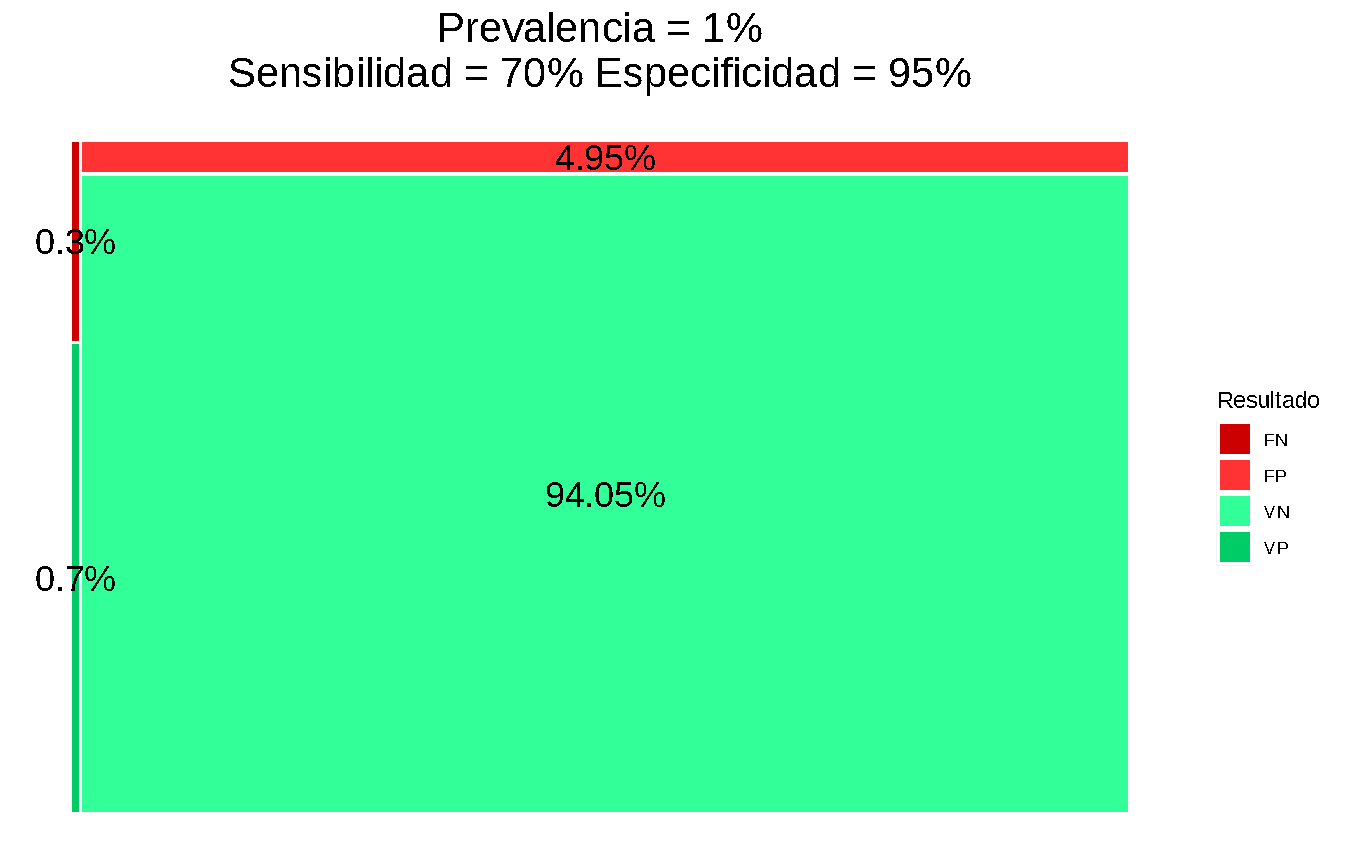
\includegraphics[width=0.85\linewidth,height=\textheight,keepaspectratio]{img/tests/resultados-test-prevalencia-1.pdf}

}

\caption{\label{fig-resultados-test-prevalencia-1}Resultados de un test
diagnóstico con una sensibilidad del 70 \%, una especificidad del 95 \%
y una prevalencia del 1 \%}

\end{figure}%

Mientras que, si la prevalencia es del 10 \%, se tiene

{\def\LTcaptype{none} % do not increment counter
\begin{longtable}[]{@{}lcc@{}}
\toprule\noalign{}
Test & \(E\) & \(\overline{E}\) \\
\midrule\noalign{}
\endhead
\bottomrule\noalign{}
\endlastfoot
Positivo \(+\) & 70 & 45 \\
Negativo \(-\) & 30 & 855 \\
\end{longtable}
}

\begin{figure}

\centering{

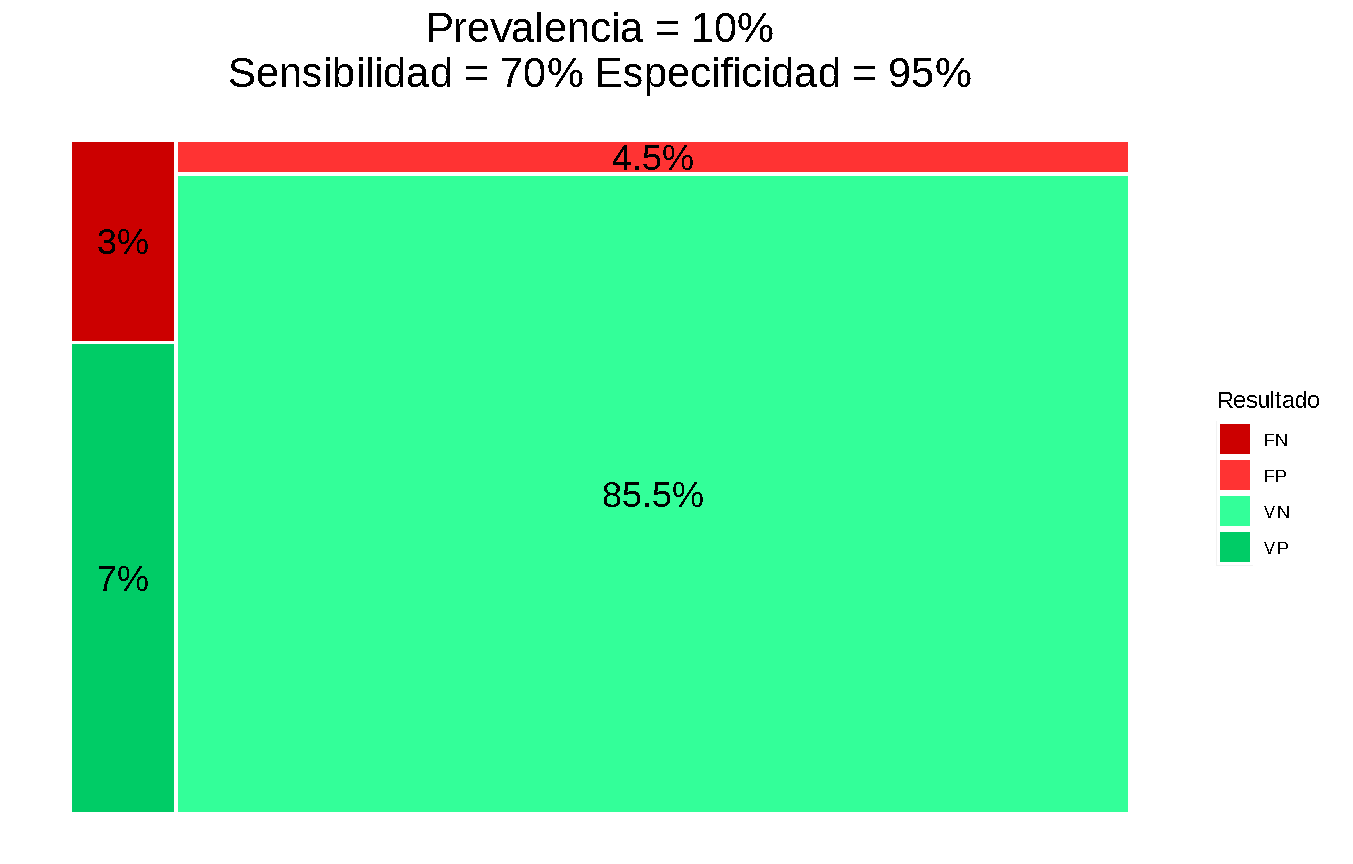
\includegraphics[width=0.85\linewidth,height=\textheight,keepaspectratio]{img/tests/resultados-test-prevalencia-10.pdf}

}

\caption{\label{fig-resultados-test-prevalencia-10}Resultados de un test
diagnóstico con una sensibilidad del 70 \%, una especificidad del 95 \%
y una prevalencia del 10 \%}

\end{figure}%

Obsérvese que, aunque la sensibilidad y la especificidad del test son
las mismas en ambos casos, con una prevalencia del 1 \% la mayoría de
los positivos del test son falsos positivos, mientras que con una
prevalencia del 10 \% la mayoría son verdaderos positivos.

\end{example}

\begin{tcolorbox}[enhanced jigsaw, arc=.35mm, bottomrule=.15mm, bottomtitle=1mm, breakable, colback=white, colbacktitle=quarto-callout-tip-color!10!white, colframe=quarto-callout-tip-color-frame, coltitle=black, left=2mm, leftrule=.75mm, opacityback=0, opacitybacktitle=0.6, rightrule=.15mm, title=\textcolor{quarto-callout-tip-color}{\faLightbulb}\hspace{0.5em}{Aplicación interactiva}, titlerule=0mm, toprule=.15mm, toptitle=1mm]

Para ver los resultados de un test diagnóstico en función de la
prevalencia, la sensibilidad y la especificidad se puede utilizar esta
\href{http://nube.aprendeconalf.es/shiny/diagnostic-test/}{aplicación
para tests diagnósticos}.

\end{tcolorbox}

\subsection{Cuándo usar un test más sensible o más
específico}\label{cuuxe1ndo-usar-un-test-muxe1s-sensible-o-muxe1s-especuxedfico}

Una mayor sensibilidad aumenta el número de verdaderos positivos y
disminuye el número de falsos negativos, mientras que una mayor
especificidad aumenta el número de verdaderos negativos y disminuye el
número de falsos positivos.

Por tanto, utilizaremos un test \textbf{más sensible} cuando:

\begin{itemize}
\tightlist
\item
  La enfermedad es grave o muy contagiosa y es importante detectarla.
\item
  La enfermedad es curable.
\item
  Los falsos positivos no provocan traumas serios.
\end{itemize}

Y utilizaremos un test \textbf{más específico} cuando:

\begin{itemize}
\tightlist
\item
  La enfermedad es importante pero difícil o imposible de curar.
\item
  Los falsos positivos pueden provocar traumas serios.
\item
  El tratamiento de los falsos positivos puede tener graves
  consecuencias.
\end{itemize}

Tanto la sensibilidad como la especificidad son indicadores de la
fiabilidad de un test \emph{a priori}, es decir, antes de aplicarlo. Una
vez que el test se ha aplicado y se conoce su resultado, a la hora de
diagnosticar la enfermedad o descartarla es mejor utilizar los
\emph{valores predictivos}.

\section{Valores predictivos de un
test}\label{valores-predictivos-de-un-test}

\begin{definition}[Valor predictivo
positivo]\protect\hypertarget{def-valor-predictivo-positivo}{}\label{def-valor-predictivo-positivo}

El \emph{valor predictivo positivo} de un test diagnóstico es la
proporción de personas con la enfermedad entre las personas con
resultado positivo en el test,

\[VPP = P(E|+) = \frac{VP}{VP+FP}\]

\end{definition}

\begin{definition}[Valor predictivo
negativo]\protect\hypertarget{def-valor-predictivo-negativo}{}\label{def-valor-predictivo-negativo}

El \emph{valor predictivo negativo} de un test diagnóstico es la
proporción de personas sin la enfermedad entre las personas con
resultado negativo en el test,

\[VPN = P(\overline{E}|-) = \frac{VN}{VN+FN}\]

\end{definition}

\begin{example}[]\protect\hypertarget{exm-valores-predictivos}{}\label{exm-valores-predictivos}

Siguiendo con el ejemplo anterior y suponiendo una prevalencia del 1 \%,
se tiene

{\def\LTcaptype{none} % do not increment counter
\begin{longtable}[]{@{}lcc@{}}
\toprule\noalign{}
Test & \(E\) & \(\overline{E}\) \\
\midrule\noalign{}
\endhead
\bottomrule\noalign{}
\endlastfoot
Positivo \(+\) & 7 & 50 \\
Negativo \(-\) & 3 & 940 \\
\end{longtable}
}

\[VPP = \frac{7}{7+50} = 0.123, \qquad VPN = \frac{940}{3+940} = 0.997.\]

Mientras que, si la prevalencia es del 10 \%, se tiene

{\def\LTcaptype{none} % do not increment counter
\begin{longtable}[]{@{}lcc@{}}
\toprule\noalign{}
Test & \(E\) & \(\overline{E}\) \\
\midrule\noalign{}
\endhead
\bottomrule\noalign{}
\endlastfoot
Positivo \(+\) & 70 & 45 \\
Negativo \(-\) & 30 & 855 \\
\end{longtable}
}

\[VPP = \frac{70}{70+45} = 0.609, \qquad VPN = \frac{855}{30+855} = 0.966.\]

\end{example}

\begin{tcolorbox}[enhanced jigsaw, arc=.35mm, bottomrule=.15mm, bottomtitle=1mm, breakable, colback=white, colbacktitle=quarto-callout-important-color!10!white, colframe=quarto-callout-important-color-frame, coltitle=black, left=2mm, leftrule=.75mm, opacityback=0, opacitybacktitle=0.6, rightrule=.15mm, title=\textcolor{quarto-callout-important-color}{\faExclamation}\hspace{0.5em}{Importante}, titlerule=0mm, toprule=.15mm, toptitle=1mm]

A diferencia de la sensibilidad y la especificidad, que son propiedades
del test, los valores predictivos dependen de la prevalencia de la
enfermedad en la población estudiada. Por eso un mismo test puede ser
muy útil en una población con prevalencia alta e inútil en una población
con prevalencia baja.

\end{tcolorbox}

\subsection{Interpretación de los valores
predictivos}\label{interpretaciuxf3n-de-los-valores-predictivos}

\begin{tcolorbox}[enhanced jigsaw, arc=.35mm, bottomrule=.15mm, bottomtitle=1mm, breakable, colback=white, colbacktitle=quarto-callout-note-color!10!white, colframe=quarto-callout-note-color-frame, coltitle=black, left=2mm, leftrule=.75mm, opacityback=0, opacitybacktitle=0.6, rightrule=.15mm, title=\textcolor{quarto-callout-note-color}{\faInfo}\hspace{0.5em}{Interpretación}, titlerule=0mm, toprule=.15mm, toptitle=1mm]

\[
\begin{array}{rcl}
VPP>0.5 & \Rightarrow & \mbox{Diagnosticar la enfermedad},\\
VPN>0.5 & \Rightarrow & \mbox{Descartar la enfermedad}.
\end{array}
\]

\end{tcolorbox}

En el ejemplo anterior, con una prevalencia del 1 \% un resultado
positivo no permite diagnosticar la enfermedad (\(VPP=0.123\)), mientras
que con una prevalencia del 10 \% sí (\(VPP=0.609\)). En ambos casos, en
cambio, un resultado negativo permite descartarla con bastante
seguridad.

\bookmarksetup{startatroot}

\chapter{La curva ROC}\label{sec-curva-roc}

En los tests diagnósticos basados en la medición de una variable
cuantitativa (como, por ejemplo, los tests de antígenos para la COVID)
la sensibilidad y la especificidad dependen del umbral fijado para dar
un positivo.

Al bajar el umbral aumenta la sensibilidad, pero disminuye la
especificidad, y al subirlo ocurre lo contrario, de manera que no es
posible resumir la fiabilidad del test con un único par de valores. Para
evaluar la fiabilidad de estos tests se suele utilizar la \emph{curva
ROC}.

\section{Definición de la curva
ROC}\label{definiciuxf3n-de-la-curva-roc}

\begin{definition}[Curva
ROC]\protect\hypertarget{def-curva-roc}{}\label{def-curva-roc}

La \emph{curva ROC} (del inglés \emph{Receiver Operating
Characteristic}) de un test diagnóstico es la curva que resulta de
representar la razón de verdaderos positivos (sensibilidad) frente a la
razón de falsos positivos (1 − especificidad) para los diferentes
umbrales de positivo del test.

\end{definition}

\begin{figure}

\centering{

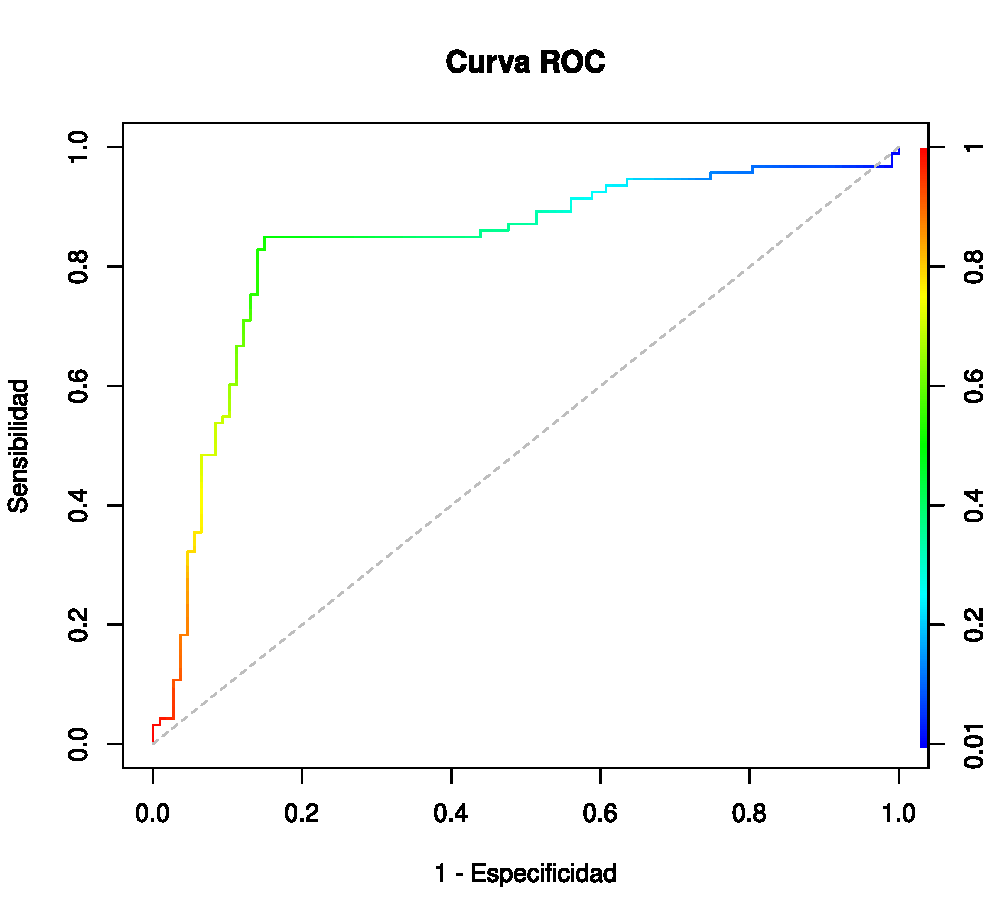
\includegraphics[width=0.65\linewidth,height=\textheight,keepaspectratio]{img/tests/curva-roc.pdf}

}

\caption{\label{fig-curva-roc}Curva ROC de un test diagnóstico}

\end{figure}%

\subsection{Interpretación de la curva
ROC}\label{interpretaciuxf3n-de-la-curva-roc}

\begin{tcolorbox}[enhanced jigsaw, arc=.35mm, bottomrule=.15mm, bottomtitle=1mm, breakable, colback=white, colbacktitle=quarto-callout-note-color!10!white, colframe=quarto-callout-note-color-frame, coltitle=black, left=2mm, leftrule=.75mm, opacityback=0, opacitybacktitle=0.6, rightrule=.15mm, title=\textcolor{quarto-callout-note-color}{\faInfo}\hspace{0.5em}{Interpretación}, titlerule=0mm, toprule=.15mm, toptitle=1mm]

\begin{itemize}
\tightlist
\item
  Cada punto de la curva corresponde a un umbral para el positivo.
\item
  El mejor test es el que se sitúa en la esquina superior izquierda del
  espacio (sensibilidad 1 y especificidad 1).
\item
  La diagonal representa un test con un diagnóstico aleatorio.
\end{itemize}

\end{tcolorbox}

Así, la curva ROC sirve también para seleccionar el umbral más adecuado
en función de si interesa priorizar la sensibilidad o la especificidad,
tal y como se explicó en el Capítulo~\ref{sec-tests-diagnosticos}.

\section{Área debajo de la curva ROC
(AUC)}\label{uxe1rea-debajo-de-la-curva-roc-auc}

Para evaluar la fiabilidad de un test diagnóstico independientemente del
umbral de positivos se suele medir el área bajo la curva ROC, también
conocida como \emph{AUC} (\emph{area under the curve}).

\begin{definition}[Área bajo la
curva]\protect\hypertarget{def-auc}{}\label{def-auc}

El \emph{área bajo la curva ROC} o \emph{AUC} es la probabilidad de que,
tomados al azar un individuo enfermo y otro sano, el test asigne al
enfermo un valor más indicativo de la enfermedad que al sano.

\end{definition}

Según el valor del AUC, se tiene:

\begin{longtable}[]{@{}cl@{}}
\caption{Interpretación del área bajo la curva
ROC}\label{tbl-auc}\tabularnewline
\toprule\noalign{}
AUC & Fiabilidad del test \\
\midrule\noalign{}
\endfirsthead
\toprule\noalign{}
AUC & Fiabilidad del test \\
\midrule\noalign{}
\endhead
\bottomrule\noalign{}
\endlastfoot
0.5 & Diagnóstico aleatorio \\
{[}0.5, 0.6) & Test malo \\
{[}0.6, 0.75) & Test regular \\
{[}0.75, 0.9) & Test bueno \\
{[}0.9, 0.97) & Test muy bueno \\
{[}0.97, 1) & Test excelente \\
\end{longtable}

\section{Aplicaciones a la COVID}\label{aplicaciones-a-la-covid}

\begin{itemize}
\tightlist
\item
  \href{https://www.rcpjournals.org/content/clinmedicine/20/6/e209}{Fiabilidad
  del diagnóstico por PCR}.
\item
  \href{https://www.cdc.gov/mmwr/volumes/69/wr/mm695152a3.htm}{Fiabilidad
  del diagnóstico por el test de antígenos}.
\item
  \href{https://academic.oup.com/ajcp/article/154/5/575/5898531}{Comparativa
  de tests}.
\end{itemize}

Los tests de antígenos son más rápidos que las PCR, pero son menos
fiables.

Por un lado, son menos sensibles que una prueba de PCR, debido a que se
requiere una mayor cantidad de virus en las mucosas nasales o bucales
para que se muestre un resultado positivo. Eso limita su efectividad
cuando las personas llevan poco tiempo infectadas y el virus está
empezando a reproducirse.

Por otro lado, también son menos específicos que la PCR y, por tanto,
producen más falsos positivos.

\cleardoublepage
\phantomsection
\addcontentsline{toc}{part}{Apéndices}
\appendix

\chapter*{Referencias}\label{sec-referencias}
\addcontentsline{toc}{chapter}{Referencias}

\markboth{Referencias}{Referencias}

\section*{Recursos generales}\label{recursos-generales}
\addcontentsline{toc}{section}{Recursos generales}

\markright{Recursos generales}

\begin{itemize}
\tightlist
\item
  \href{http://matematicas.uclm.es/cemat/covid19/}{Acción matemática
  contra el coronavirus}.
\item
  \href{https://www.repidemicsconsortium.org/}{R Epidemic Consortium
  (RECON)}.
\item
  \href{https://cran.r-project.org/doc/contrib/Epicalc_Book.pdf}{Analysis
  of epidemiological data using R and Epicalc}.
\item
  \href{https://statsandr.com/blog/top-r-resources-on-covid-19-coronavirus/\#coronavirus}{R
  resources about COVID-19}.
\end{itemize}

\section*{Datos epidemiológicos}\label{datos-epidemioluxf3gicos}
\addcontentsline{toc}{section}{Datos epidemiológicos}

\markright{Datos epidemiológicos}

\begin{itemize}
\tightlist
\item
  \href{https://www.sanidad.gob.es/profesionales/saludPublica/ccayes/alertasActual/nCov/situacionActual.htm}{Situación
  actual de la COVID-19 (Ministerio de Sanidad)}.
\item
  \href{https://www.isciii.es/QueHacemos/Servicios/VigilanciaSaludPublicaRENAVE/Paginas/default.aspx}{Centro
  Nacional de Epidemiología (Instituto de Salud Carlos III)}.
\item
  \href{https://www.ecdc.europa.eu/en/data}{European Centre for Disease
  Prevention and Control (ECDC)}.
\item
  \href{https://www.who.int/data}{World Health Organization (WHO)}.
\end{itemize}

\section*{Aplicaciones interactivas}\label{aplicaciones-interactivas}
\addcontentsline{toc}{section}{Aplicaciones interactivas}

\markright{Aplicaciones interactivas}

\begin{itemize}
\tightlist
\item
  \href{http://nube.aprendeconalf.es/shiny/diagnostic-test/}{Aplicación
  para el estudio de tests diagnósticos}.
\end{itemize}

\section*{Otros manuales del autor}\label{otros-manuales-del-autor}
\addcontentsline{toc}{section}{Otros manuales del autor}

\markright{Otros manuales del autor}

\begin{itemize}
\tightlist
\item
  \href{https://aprendeconalf.es/estadistica-manual/}{Manual de
  Estadística}.
\item
  \href{https://aprendeconalf.es/estadistica-ejercicios/}{Colección de
  problemas resueltos de Estadística}.
\item
  \href{https://aprendeconalf.es/estadistica-practicas-r/}{Prácticas de
  Estadística con R}.
\end{itemize}




\end{document}
